\documentclass[11pt,a4paper]{article}
\usepackage[utf8]{inputenc}
\usepackage[T1]{fontenc}
\usepackage{amsmath,amssymb}
\usepackage{graphicx}
\usepackage{booktabs}
\usepackage{hyperref}
\usepackage{subcaption}
\usepackage{float}
\usepackage[margin=2.5cm]{geometry}

\title{Element Learning: Numerical Experiments Report\\
\large 1D Burgers, 2D Linear Wave, 2D Nonlinear Shallow Water}
\author{}
\date{\today}

\begin{document}
\maketitle

\begin{abstract}
We report numerical experiments for data-driven surrogate models of three PDEs: (1)~1D viscous Burgers equation (finite-volume reference vs.\ MLP); (2)~2D linear wave equation (Fourier spectral reference vs.\ MLP); (3)~2D nonlinear shallow water (Fourier spectral reference vs.\ CNN). For each problem we generate training data from the reference solver, train a neural network, and compare reference and NN rollouts in time. Training curves and comparison figures are included.
\end{abstract}

\section{Background}

\subsection{Element learning}
The goal is to learn a local map on a small spatial element or patch from data produced by a high-fidelity solver. At inference time, the learned map is applied in rollout form over the full domain, yielding a fast surrogate that can be compared to the reference solver in both accuracy and runtime.

\subsection{Three test cases}
\begin{itemize}
  \item \textbf{1D Burgers (viscous):} $u_t + u u_x = \nu u_{xx}$ on $[0,L]$ with periodic BC. Reference: finite-volume Godunov flux with implicit diffusion. NN: MLP mapping a 1D patch to the interior window over one NN step.
  \item \textbf{2D linear wave:} $u_{tt} = c^2(u_{xx}+u_{yy})$ with periodic BC. Reference: Fourier pseudo-spectral with RK4 time stepping. NN: MLP mapping patch data from displacement and velocity channels to the interior window.
  \item \textbf{2D nonlinear shallow water:} state $(h,q_x,q_y)$ solved by a spectral reference model. NN: CNN patch-to-patch predictor trained with per-channel relative TV regularization.
\end{itemize}

\section{Experimental parameters}

\subsection{1D Burgers}
\begin{table}[H]
  \centering
  \caption{Burgers configuration from \texttt{config/burgers\_1d\_config.py}.}
  \begin{tabular}{ll}
    \toprule
    Parameter & Value \\
    \midrule
    Domain length $L$ & 2.0 \\
    Grid cells $n_x$ & 2000 \\
    CFL & 0.5 \\
    Patch half-width $n_{\mathrm{st}}$ & 51 \\
    Interior width $n_{\mathrm{wd}}$ & 100 \\
    Jumps per NN step $n_{\mathrm{jp}}$ & 100 \\
    Viscosity $\nu$ & $10^{-3}$ \\
    IC decay $\alpha$ & 2.5 \\
    Training samples & 5000 \\
    Batch size & 128 \\
    Epochs & 2500 \\
    Hidden size / layers & 128 / 5 \\
    Activation & ReLU \\
    \bottomrule
  \end{tabular}
\end{table}

\subsection{2D linear wave}
\begin{table}[H]
  \centering
  \caption{Linear wave configuration from \texttt{config/wave\_2d\_linear\_config.py}.}
  \begin{tabular}{ll}
    \toprule
    Parameter & Value \\
    \midrule
    Grid $N_X\times N_Y$ & $256\times256$ \\
    Domain $L_x=L_y$ & $2\pi$ \\
    $\Delta t$ & $2\times 10^{-3}$ \\
    Wave speed $c$ & 1.0 \\
    Steps per saved frame $T_{\mathrm{screen}}$ & 50 \\
    Frames per NN step $n_{\mathrm{jp}}$ & 2 \\
    Patch half-width $n_{\mathrm{st}}$ & 9 \\
    Interior width $n_{\mathrm{wd}}$ & 32 \\
    Training samples & 5000 \\
    Epochs & 2500 \\
    Hidden size / layers & 256 / 1 \\
    Activation & linear \\
    Compare IC & ring \\
    \bottomrule
  \end{tabular}
\end{table}

\subsection{2D nonlinear shallow water}
\begin{table}[H]
  \centering
  \caption{Nonlinear shallow-water configuration from \texttt{config/wave\_2d\_nonlinear\_config.py}.}
  \begin{tabular}{ll}
    \toprule
    Parameter & Value \\
    \midrule
    Grid $n_x\times n_y$ & $256\times256$ \\
    Domain $L_x=L_y$ & $2\pi$ \\
    $g$, $h_0$ & 9.8, 1.0 \\
    Time integrator & IMEX (Strang splitting) \\
    Time step $\Delta t$ & $0.5\min(\Delta x,\Delta y)$ \\
    Steps per saved frame $T_{\mathrm{screen}}$ & 4 \\
    Patch half-width $n_{\mathrm{st}}$ & 8 \\
    Interior width $n_{\mathrm{wd}}$ & 16 \\
    Viscosity $\nu_h$ & 0 \\
    Nudging coefficient & 1.0 \\
    Batch size & 100 \\
    Warmup time & 5.0 \\
    Compare $T_F$ & 2.0 \\
    Compare frames & 8 \\
    Compare IC & random \\
    Training samples & 3000 \\
    Epochs & 150 \\
    CNN base channels & 64 \\
    TV smooth weight & [1e-2, 0, 0] \\
    TV smooth mode & absolute \\
    Data loss channel weights & [10, 1, 1] \\
    \bottomrule
  \end{tabular}
\end{table}

\section{Results}

\subsection{Training history}
Figure~\ref{fig:training} shows the train and test loss versus epoch for the three problems.

\begin{figure}[H]
  \centering
  \begin{subfigure}[t]{0.32\textwidth}
    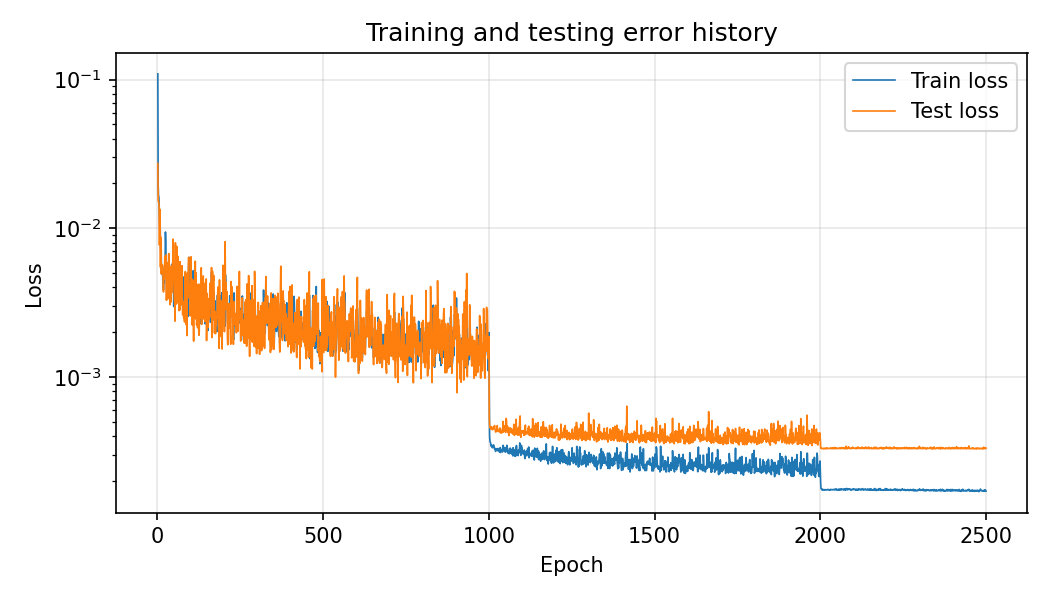
\includegraphics[width=\textwidth]{figures/burgers_1d/training_history.png}
    \caption{Burgers 1D}
  \end{subfigure}
  \hfill
  \begin{subfigure}[t]{0.32\textwidth}
    
\includegraphics[width=\textwidth]{figures/wave_2d_linear/training_history.png}
    \caption{2D linear wave}
  \end{subfigure}
  \hfill
  \begin{subfigure}[t]{0.32\textwidth}
    
\includegraphics[width=\textwidth]{figures/wave_2d_nonlinear/training_history.png}
    \caption{2D nonlinear}
  \end{subfigure}
  \caption{Training and test loss versus epoch.}
  \label{fig:training}
\end{figure}

\subsection{1D Burgers: FV vs. NN}
Comparison at 6 output times over $t\in[0,2]$ with \texttt{compare\_t\_end=2.0}. Runtime for this run: FV total $4.081$\,s, NN total $0.3124$\,s, speedup $13.1\times$.

\begin{figure}[H]
  \centering
  
\includegraphics[width=0.7\textwidth]{figures/burgers_1d/t0.png}
  \caption{Burgers: initial frame.}
\end{figure}
\begin{figure}[H]
  \centering
  
\includegraphics[width=0.7\textwidth]{figures/burgers_1d/t2.png}
  \caption{Burgers: mid-run frame.}
\end{figure}
\begin{figure}[H]
  \centering
  
\includegraphics[width=0.7\textwidth]{figures/burgers_1d/t5.png}
  \caption{Burgers: final frame.}
\end{figure}

\subsection{2D linear wave: Spectral vs. NN}
Comparison at 6 aligned frames with \texttt{compare\_TF=2.0} and \texttt{compare\_ic=ring}. Runtime for this run: spectral $6.509$\,s, NN $0.1712$\,s, speedup $38.0\times$.

\begin{figure}[H]
  \centering
  
\includegraphics[width=0.85\textwidth]{figures/wave_2d_linear/t0.png}
  \caption{2D linear wave: initial frame.}
\end{figure}
\begin{figure}[H]
  \centering
  
\includegraphics[width=0.85\textwidth]{figures/wave_2d_linear/t3.png}
  \caption{2D linear wave: mid-run frame.}
\end{figure}
\begin{figure}[H]
  \centering
  
\includegraphics[width=0.85\textwidth]{figures/wave_2d_linear/t5.png}
  \caption{2D linear wave: final frame.}
\end{figure}

\subsection{2D nonlinear shallow water: Spectral vs. NN}
Comparison at 8 aligned frames for $(h-h_0,q_x,q_y)$ with \texttt{compare\_TF=2.0} and \texttt{compare\_ic=random}. Both rollouts start after warmup time $T=5.0$. Final rollout metrics for this run: mean L1 error $0.009446$, max-frame L1 error $0.016583$, spectral runtime $25.041$\,s, NN runtime $2.2758$\,s, speedup $11.0\times$.

\begin{figure}[H]
  \centering
  
\includegraphics[width=0.9\textwidth]{figures/wave_2d_nonlinear/t0.png}
  \caption{2D nonlinear shallow water: initial frame.}
\end{figure}
\begin{figure}[H]
  \centering
  
\includegraphics[width=0.9\textwidth]{figures/wave_2d_nonlinear/t3.png}
  \caption{2D nonlinear shallow water: mid-run frame.}
\end{figure}
\begin{figure}[H]
  \centering
  
\includegraphics[width=0.9\textwidth]{figures/wave_2d_nonlinear/t7.png}
  \caption{2D nonlinear shallow water: final frame.}
\end{figure}

\section{Conclusion}
The three pipelines run successfully with a unified workflow: \texttt{gen\_data.py}, \texttt{python -m ml.train}, and \texttt{compare.py} are all selected through the shared \texttt{--problem} interface. The rebuilt figures show that the learned surrogates track the reference solutions while delivering clear runtime savings in all three cases.

\end{document}
